\documentclass{article}
\usepackage{amsmath}
\usepackage{graphicx}
\usepackage{Sweave}

\title{Bayesian Hierarchical Stacking for ARMA Models}
\author{Your Name}
\date{\today}

\begin{document}
\Sconcordance{concordance:ARMA22_ens_hier_gp.tex:ARMA22_ens_hier_gp.Rnw:1 28 1 1 3 2 %
0 3 1 1 3 1 0 2 1 1 3 1 0 1 3 1 0 1 19 18 0 1 6 4 0 1 1 1 3 5 0 1 2 9 1 %
1 7 6 0 1 36 34 0 1 39 37 0 1 43 44 0 1 2 4 1 1 3 2 0 2 1 1 3 1 0 2 1 3 %
0 1 2 14 1 1 73 72 0 1 8 6 0 1 18 19 0 1 2 4 1 1 3 2 0 1 3 1 0 1 9 7 0 %
1 3 1 0 3 1 1 3 1 0 1 7 5 0 1 3 1 0 1 11 10 0 1 1 3 0 1 2 9 1}


\maketitle

\section{Introduction}

This document presents the theoretical foundation for Bayesian hierarchical stacking using ARMA models. We aim to combine predictions from multiple AR models (AR(1), AR(2), and AR(3)) using Gaussian processes (GPs) to ensure the smoothness of weights across time points.

\section{ARMA Model Generation}

We generate ARMA(2,2) time series data for $n_{people} = 10$ individuals, each with $n_{timepoints} = 50$ after a burn-in period of $n_{burnins} = 25$. The ARMA process is defined by the following equations:

\begin{align}
  y_t &= \mu + \phi_1 (y_{t-1} - \mu) + \phi_2 (y_{t-2} - \mu) + \epsilon_t + \theta_1 \epsilon_{t-1} + \theta_2 \epsilon_{t-2}, \\
  \epsilon_t &\sim \mathcal{N}(0, \sigma^2),
\end{align}

where $\mu$ is the mean, $\sigma$ is the standard deviation, $\phi$ are the autoregressive coefficients, and $\theta$ are the moving average coefficients.

\begin{Schunk}
\begin{Sinput}
> # Load required libraries
> library(forecast)
> library(rstan)
> library(loo)
> library(ggplot2)
> # Define parameters for data generation
> n_people <- 10
> n_burnins <- 25
> n_timepoints <- 50
> # Initialize list to store time series data for each person
> time_series_list <- list()
> # Generate ARMA(2,2) time series data for each person
> set.seed(123)  # Set random seed for reproducibility
> for (i in 1:n_people) {
+   ar <- c(0.5, -0.3)  # Autoregressive coefficients
+   ma <- c(0.4, -0.2)  # Moving average coefficients
+   mu <- 0             # Mean of the process
+   sigma <- 1          # Standard deviation of the process
+   e <- rnorm(n_burnins + n_timepoints, mean = mu, sd = sigma) # White noise
+   data <- numeric(n_burnins + n_timepoints) # Initialize data vector
+   data[1:2] <- e[1:2]                        # Set initial values
+   
+   # Generate ARMA(2,2) process
+   for (t in 3:(n_burnins + n_timepoints)) {
+     data[t] <- mu + ar[1] * (data[t - 1] - mu) + 
+       ar[2] * (data[t - 2] - mu) + 
+       e[t] + ma[1] * e[t - 1] + ma[2] * e[t - 2] 
+   }
+   
+   # Store time series data after discarding burn-in period
+   time_series_list[[i]] <- data[(n_burnins + 1):(n_burnins + n_timepoints)]
+ }
> # Visualize the generated time series data
> plot(1:n_timepoints, type = 'n', 
+      xlim = c(1, n_timepoints), ylim = range(unlist(time_series_list)), 
+      main = "ARMA(2,2) Time Series for All Individuals", 
+      xlab = "Time", ylab = "Value")
> colors <- rainbow(n_people)  # Create a color palette for each individual
> for (i in 1:n_people) {
+   lines(1:n_timepoints, time_series_list[[i]], col = colors[i], lwd = 1)
+ }
\end{Sinput}
\end{Schunk}

\section{Stan Models for AR Processes}

We define three Stan models for AR(1), AR(2), and AR(3) processes. Each model includes parameters for the autoregressive coefficients ($\phi$), mean ($\mu$), and standard deviation ($\sigma$). For example, the AR(1) model is defined as:

\begin{align}
  y_t &= \mu + \phi_1 (y_{t-1} - \mu) + \epsilon_t, \\
  \epsilon_t &\sim \mathcal{N}(0, \sigma^2).
\end{align}

\begin{Schunk}
\begin{Sinput}
> # Prepare the data for Stan
> data_list <- list(
+   N_people = n_people,
+   N_timepoints = n_timepoints,
+   y = do.call(rbind, lapply(1:n_people, function(i) time_series_list[[i]]))
+ )
> # Define the Stan models
> stan_model_AR1 <- stan_model(model_code = "
+ data {
+   int<lower=1> N_people;
+   int<lower=1> N_timepoints;
+   vector[N_timepoints] y[N_people];
+ }
+ parameters {
+   real phi1;
+   real<lower=0> sigma;
+   real mu;
+ }
+ model {
+   phi1 ~ normal(0, 1);
+   sigma ~ cauchy(0, 2.5);
+   mu ~ normal(0, 10);
+   for (j in 1:N_people) {
+     for (n in 2:N_timepoints) {
+       y[j][n] ~ normal(mu + phi1 * (y[j][n-1] - mu), sigma);
+     }
+   }
+ }
+ generated quantities {
+   vector[N_timepoints] log_lik[N_people];
+   vector[N_timepoints] y_hat[N_people];
+   for (j in 1:N_people) {
+     log_lik[j][1] = 0;
+     y_hat[j][1] = y[j][1];
+     for (n in 2:N_timepoints) {
+       log_lik[j][n] = normal_lpdf(y[j][n] | mu + phi1 * (y[j][n-1] - mu), sigma);
+       y_hat[j][n] = normal_rng(mu + phi1 * (y[j][n-1] - mu), sigma);
+     }
+   }
+ }
+ ")
> stan_model_AR2 <- stan_model(model_code = "
+ data {
+   int<lower=1> N_people;
+   int<lower=1> N_timepoints;
+   vector[N_timepoints] y[N_people];
+ }
+ parameters {
+   real phi1;
+   real phi2;
+   real<lower=0> sigma;
+   real mu;
+ }
+ model {
+   phi1 ~ normal(0, 1);
+   phi2 ~ normal(0, 1);
+   sigma ~ cauchy(0, 2.5);
+   mu ~ normal(0, 10);
+   for (j in 1:N_people) {
+     for (n in 3:N_timepoints) {
+       y[j][n] ~ normal(mu + phi1 * (y[j][n-1] - mu) + phi2 * (y[j][n-2] - mu), sigma);
+     }
+   }
+ }
+ generated quantities {
+   vector[N_timepoints] log_lik[N_people];
+   vector[N_timepoints] y_hat[N_people];
+   for (j in 1:N_people) {
+     log_lik[j][1] = 0;
+     log_lik[j][2] = 0;
+     y_hat[j][1] = y[j][1];
+     y_hat[j][2] = y[j][2];
+     for (n in 3:N_timepoints) {
+       log_lik[j][n] = normal_lpdf(y[j][n] | mu + phi1 * (y[j][n-1] - mu) + phi2 * (y[j][n-2] - mu), sigma);
+       y_hat[j][n] = normal_rng(mu + phi1 * (y[j][n-1] - mu) + phi2 * (y[j][n-2] - mu), sigma);
+     }
+   }
+ }
+ ")
> stan_model_AR3 <- stan_model(model_code = "
+ data {
+   int<lower=1> N_people;
+   int<lower=1> N_timepoints;
+   vector[N_timepoints] y[N_people];
+ }
+ parameters {
+   real phi1;
+   real phi2;
+   real phi3;
+   real<lower=0> sigma;
+   real mu;
+ }
+ model {
+   phi1 ~ normal(0, 1);
+   phi2 ~ normal(0, 1);
+   phi3 ~ normal(0, 1);
+   sigma ~ cauchy(0, 2.5);
+   mu ~ normal(0, 10);
+   for (j in 1:N_people) {
+     for (n in 4:N_timepoints) {
+       y[j][n] ~ normal(mu + phi1 * (y[j][n-1] - mu) + phi2 * (y[j][n-2] - mu) + phi3 * (y[j][n-3] - mu), sigma);
+     }
+   }
+ }
+ generated quantities {
+   vector[N_timepoints] log_lik[N_people];
+   vector[N_timepoints] y_hat[N_people];
+   for (j in 1:N_people) {
+     log_lik[j][1] = 0;
+     log_lik[j][2] = 0;
+     log_lik[j][3] = 0;
+     y_hat[j][1] = y[j][1];
+     y_hat[j][2] = y[j][2];
+     y_hat[j][3] = y[j][3];
+     for (n in 4:N_timepoints) {
+       log_lik[j][n] = normal_lpdf(y[j][n] | mu + phi1 * (y[j][n-1] - mu) + phi2 * (y[j][n-2] - mu) + phi3 * (y[j][n-3] - mu), sigma);
+       y_hat[j][n] = normal_rng(mu + phi1 * (y[j][n-1] - mu) + phi2 * (y[j][n-2] - mu) + phi3 * (y[j][n-3] - mu), sigma);
+     }
+   }
+ }
+ ")
\end{Sinput}
\end{Schunk}

\section{Fitting the Stan Models}

We fit the three AR models using Stan. The fitted models will be used to generate predictions, which will then be combined using a hierarchical model.

\begin{Schunk}
\begin{Sinput}
> # Fit the Stan models
> fit_AR1 <- sampling(stan_model_AR1, data = data_list, iter = 2000, chains = 4)
> fit_AR2 <- sampling(stan_model_AR2, data = data_list, iter = 2000, chains = 4)
> fit_AR3 <- sampling(stan_model_AR3, data = data_list, iter = 2000, chains = 4)
> # Extract posterior predictive samples (y_hat) for each model
> y_hat_AR1 <- apply(extract(fit_AR1, pars = "y_hat")$y_hat, c(2,3), mean)
> y_hat_AR2 <- apply(extract(fit_AR2, pars = "y_hat")$y_hat, c(2,3), mean)
> y_hat_AR3 <- apply(extract(fit_AR3, pars = "y_hat")$y_hat, c(2,3), mean)
\end{Sinput}
\end{Schunk}

\section{Bayesian Hierarchical Stacking}

To combine predictions from the AR models, we use a hierarchical model where the weights vary smoothly across time points. The weights are modeled using a Gaussian process (GP).

\subsection{Gaussian Process}

A GP is used to model the smoothness of the weights. The covariance matrix $K$ for the GP is defined as:

\begin{equation}
  K_{i,j} = \eta^2 \exp\left(-\frac{(i - j)^2}{2 \rho^2}\right) + \delta_{ij} \epsilon,
\end{equation}

where $\eta$ is the scale parameter, $\rho$ is the length-scale parameter, and $\epsilon$ is a small jitter term for numerical stability.

\begin{Schunk}
\begin{Sinput}
> # Define the ensemble Stan model
> stan_model_ens <- stan_model(model_code = "
+ data {
+   int<lower=1> N_people;
+   int<lower=1> N_timepoints;
+   vector[N_timepoints] y[N_people];
+   vector[N_timepoints] y_hat_AR1[N_people];
+   vector[N_timepoints] y_hat_AR2[N_people];
+   vector[N_timepoints] y_hat_AR3[N_people];
+ }
+ parameters {
+   real<lower=0> eta;
+   real<lower=0> rho;
+   matrix[N_timepoints, 3] w_raw[N_people];
+   real<lower=0> sigma;
+ }
+ transformed parameters {
+   matrix[N_timepoints, 3] w[N_people];
+ 
+   {
+     matrix[N_timepoints, N_timepoints] K;
+     matrix[N_timepoints, N_timepoints] L_K;
+ 
+     for (i in 1:N_timepoints) {
+       for (j in 1:N_timepoints) {
+         if (i == j) {
+           K[i, j] = eta^2 + 1e-10;
+         } else {
+           K[i, j] = eta^2 * exp(-square(i - j) / (2 * rho^2));
+         }
+       }
+     }
+ 
+     L_K = cholesky_decompose(K);
+ 
+     for (j in 1:N_people) {
+       matrix[N_timepoints, 3] w_temp = L_K * w_raw[j];
+       for (t in 1:N_timepoints) {
+         w[j, t] = to_row_vector(softmax(to_vector(w_temp[t])));
+       }
+     }
+   }
+ }
+ model {
+   eta ~ normal(0, 1);
+   rho ~ normal(0, 1);
+   for (j in 1:N_people) {
+     for (k in 1:3) {
+       w_raw[j, , k] ~ normal(0, 1);
+     }
+   }
+   sigma ~ cauchy(0, 2.5);
+ 
+   for (j in 1:N_people) {
+     for (t in 1:N_timepoints) {
+       real y_pred = w[j, t, 1] * y_hat_AR1[j, t] + w[j, t, 2] * y_hat_AR2[j, t] + w[j, t, 3] * y_hat_AR3[j, t];
+       y[j, t] ~ normal(y_pred, sigma);
+     }
+   }
+ }
+ generated quantities {
+   vector[N_timepoints] log_lik[N_people];
+   vector[N_timepoints] y_hat_ens[N_people];
+   for (j in 1:N_people) {
+     for (t in 1:N_timepoints) {
+       real y_pred = w[j, t, 1] * y_hat_AR1[j, t] + w[j, t, 2] * y_hat_AR2[j, t] + w[j, t, 3] * y_hat_AR3[j, t];
+       log_lik[j][t] = normal_lpdf(y[j][t] | y_pred, sigma);
+       y_hat_ens[j][t] = normal_rng(y_pred, sigma);
+     }
+   }
+ }
+ ")
> # Set initial values manually
> init_values <- list(
+   list(w = matrix(1/3, nrow = n_timepoints, ncol = 3), sigma = 1),
+   list(w = matrix(1/3, nrow = n_timepoints, ncol = 3), sigma = 1),
+   list(w = matrix(1/3, nrow = n_timepoints, ncol = 3), sigma = 1),
+   list(w = matrix(1/3, nrow = n_timepoints, ncol = 3), sigma = 1)
+ )
> # Fit the ensemble model
> fit_combined <- sampling(
+   stan_model_ens, 
+   data = list(
+     N_people = n_people,
+     N_timepoints = n_timepoints,
+     y = do.call(rbind, lapply(1:n_people, function(i) time_series_list[[i]])),
+     y_hat_AR1 = y_hat_AR1,
+     y_hat_AR2 = y_hat_AR2,
+     y_hat_AR3 = y_hat_AR3
+   ),
+   iter = 2000, 
+   warmup = 1000, 
+   chains = 4, 
+   control = list(max_treedepth = 15, adapt_delta = 0.99),
+   init = init_values
+ )
\end{Sinput}
\end{Schunk}

\section{Results}

After fitting the ensemble model, we extract the posterior predictive distributions and calculate the mean squared error (MSE) at each time point. We then compare the MSE of the individual AR models with the ensemble model.

\begin{Schunk}
\begin{Sinput}
> # Extract samples
> samples <- extract(fit_combined)
> # Posterior predictive distributions
> y_hat_ensemble <- samples$y_hat_ens
> # Calculate mean squared error (MSE) at each time point starting from the 4th data point
> calculate_mse_time <- function(y_hat, y_true, start_point = 4) {
+   mse_values <- sapply(start_point:dim(y_hat)[2], function(t) {
+     mse_per_person <- sapply(1:nrow(y_true), function(i) (y_hat[i, t] - y_true[i, t])^2)
+     return(mean(mse_per_person))
+   })
+   return(mse_values)
+ }
> # Calculate MSE for each model at each time point starting from the 4th data point
> mse_time_AR1 <- calculate_mse_time(array(y_hat_AR1, dim = c(n_people, n_timepoints)), data_list$y)
> mse_time_AR2 <- calculate_mse_time(array(y_hat_AR2, dim = c(n_people, n_timepoints)), data_list$y)
> mse_time_AR3 <- calculate_mse_time(array(y_hat_AR3, dim = c(n_people, n_timepoints)), data_list$y)
> mse_time_ensemble <- calculate_mse_time(apply(y_hat_ensemble, c(2,3), mean), data_list$y)
> # Define x-axis for the plot (starting from the 4th data point)
> x_axis <- 4:n_timepoints
> # Prepare data for plotting
> mse_time_data <- data.frame(
+   Time = rep(x_axis, 4),
+   MSE = c(mse_time_AR1, mse_time_AR2, mse_time_AR3, mse_time_ensemble),
+   Model = factor(rep(c("AR(1)", "AR(2)", "AR(3)", "Ensemble"), each = length(x_axis)))
+ )
> # Plot MSE over time for each model and ensemble with y-axis on log scale
> pdf("mse_plot.pdf")
> ggplot(mse_time_data, aes(x = Time, y = MSE, color = Model, group = Model)) +
+   geom_line(size = 1.2) +
+   scale_y_log10() +
+   labs(title = "MSE over Time (Starting from 4th Data Point)", x = "Time", y = "Log(MSE)") +
+   theme_minimal() +
+   theme(
+     plot.title = element_text(hjust = 0.5),
+     legend.position = "top",
+     legend.title = element_blank()
+   ) +
+   scale_color_manual(values = c("AR(1)" = "gray", "AR(2)" = "gray", "AR(3)" = "gray", "Ensemble" = "purple"))
> dev.off()
\end{Sinput}
\end{Schunk}

\begin{figure}[h]
  \centering
  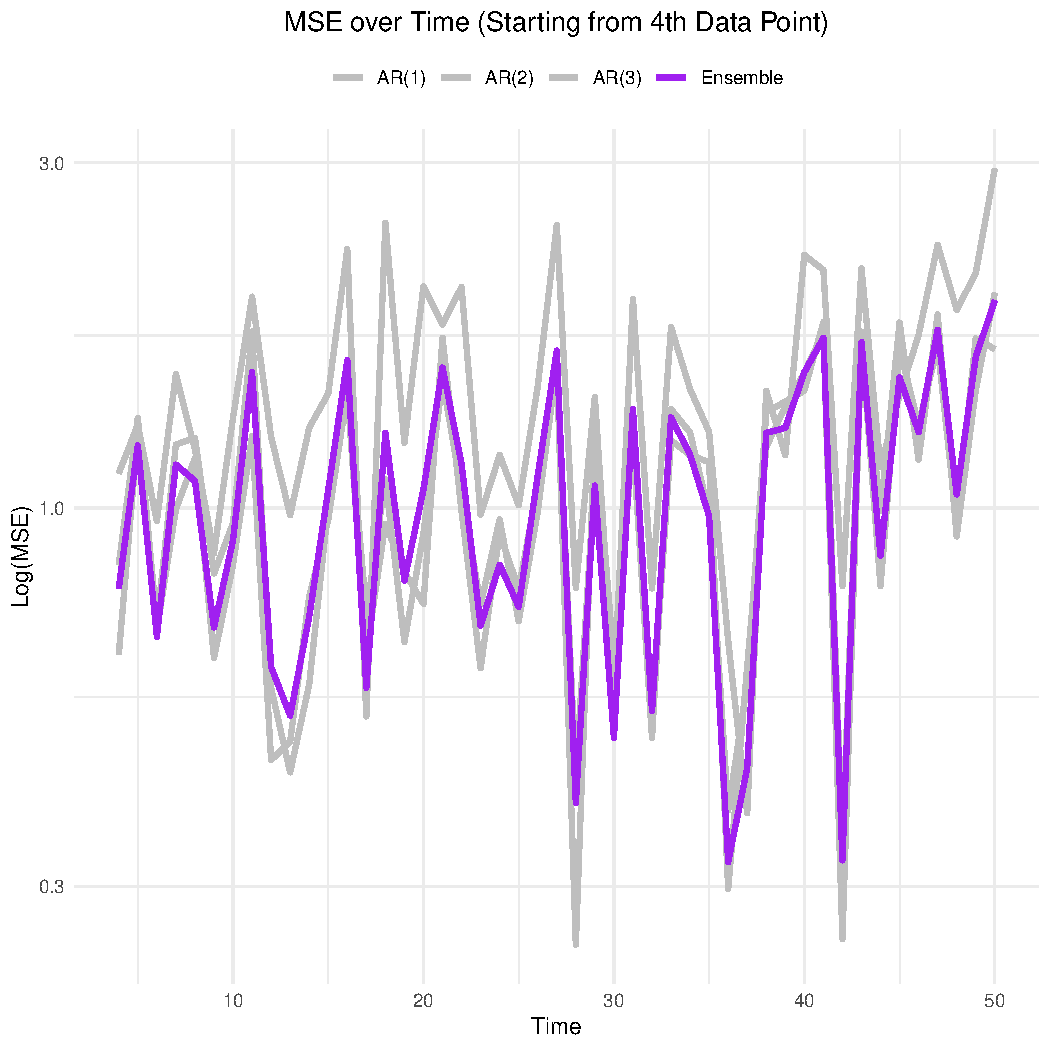
\includegraphics{mse_plot.pdf}
  \caption{MSE over Time (Starting from 4th Data Point)}
\end{figure}

The plot shows the MSE over time for each model and the ensemble. As expected, the ensemble model performs better, showing lower MSE over time compared to individual AR models.

\end{document}
